\documentclass{assignment}
\UsingEnglish
\ProjectInfos*{Intro to Communication System}{EE140}{Fall, 2020}{Assignment 1}{Due time : 10:15, Sept 18, 2020 (Friday)}{陈稼霖}{45875852}
\begin{document}
\begin{prob}[15 pts]
    Classify each of the following signals as an energy signal or as a power signal by calculating E (energy) or P (power). Note: the parameters involved are positive constants.
    \begin{itemize}
        \item[a)] $x(t)=e^{-\alpha\abs{t}}\cos\pi t$,
        \item[b)] $x(t)=\Pi(t-3)\cos 3\pi t$, $\left(\Pi(t)=\left\{\begin{array}{ll}1,&\abs{t}\leq 0.5\\0,&\text{otherwise}\end{array}\right.\right)$
        \item[c)] $x(t)=\abs{t}$,
        \item[d)] $x(t)=\sum_{n=-\infty}^{\infty}\Lambda(\frac{t}{2}-n)$, $\left(\Lambda(t)=\left\{\begin{array}{ll}1-\abs{t},&\abs{t}\\0,&\text{otherwise}\end{array}\right.\right)$
        \item[e)] $x(t)=e^{j2\pi 3t}u(t)$, $\left(u(t)=\left\{\begin{array}{ll}1,&t\geq 0\\0,&\text{otherwise}\end{array}\right.\right)$
    \end{itemize}
\end{prob}
\begin{sol}
    \begin{itemize}
        \item[a)] The energy of the signal:
        \begin{align}
            \notag E=&\int_{-\infty}^{+\infty}\abs{x(t)}^2\,dt=\int_{-\infty}^{+\infty}e^{-2\alpha\abs{t}}\cos^2\pi t\,dt\\
            \notag=&2\int_0^{+\infty}e^{-2\alpha t}\cos^2\pi t\,dt\\
            \notag=&\int_0^{+\infty}e^{-2\alpha t}(\cos 2\pi t+1)\,dt\\
            \notag=&\int_0^{+\infty}e^{-2\alpha t}\re[e^{i2\pi t}]\,dt-\left.\frac{1}{2\alpha}e^{-2\alpha t}\right\lvert_{0}^{+\infty}\\
            \notag=&\re\left[\int_0^{+\infty}e^{(-2\alpha+i2\pi)t}\,dt\right]+\frac{1}{2\alpha}\\
            \notag=&\re\left[\frac{1}{2\alpha-i2\pi}\right]+\frac{1}{2\alpha}\\
            =&\frac{\alpha}{2(\alpha^2+\pi^2)}+\frac{1}{2\alpha}<+\infty.
        \end{align}
        Therefore, the signal is \textbf{an energy signal}.
        \item[b)] The energy of the signal:
        \begin{align}
            \notag E=&\int_{-\infty}^{+\infty}\abs{x(t)}^2\,dt=\int_{-\infty}^{+\infty}\abs{\Pi(t-3)\cos 3\pi t}^2\,dt\\
            \notag=&\int_{5/2}^{7/2}\cos^23\pi t\,dt\\
            \notag=&\frac{1}{2}\int_{5/2}^{7/2}(\cos 6\pi t+1)\,dt\\
            \notag=&\frac{1}{2}\left[\frac{\sin(7/2)-\sin(5/2)}{6\pi}+1\right]<+\infty.
        \end{align}
        Therefore, the signal is \textbf{an energy signal}.
        \item[c)] The average power of the signal is
        \begin{align}
            P=\lim_{T\rightarrow+\infty}\frac{1}{T}\int_{-T/2}^{T/2}\abs{x(t)}^2\,dt=\lim_{T\rightarrow+\infty}\frac{1}{T}\int_{-T/2}^{T/2}\abs{t}^2\,dt=\lim_{T\rightarrow+\infty}\frac{2}{T}\int_0^{T/2}t^2\,dt=\lim_{T\rightarrow+\infty}\frac{T^2}{12}=+\infty.
        \end{align}
        Therefore, the signal is \textbf{neither an energy signal nor a power signal}.
        \item[d)] The signal function can be written as
        \begin{align}
            x(t)=1.
        \end{align}
        The average power of the signal:
        \begin{gather}
            P=\lim_{T\rightarrow+\infty}\frac{1}{T}\int_{-T/2}^{T/2}\abs{x(t)}^2\,dt=\lim_{T\rightarrow+\infty}\frac{1}{T}\int_{-T/2}^{T/2}\,dt=1,\\
            \Longrightarrow 0<P<+\infty.
        \end{gather}
        Therefore, the signal is \textbf{a power signal}.
        \item[e)] The average power of the signal:
        \begin{align}
            \notag P=&\lim_{T\rightarrow+\infty}\frac{1}{T}\int_{-T/2}^{T/2}\abs{x(t)}^2\,dt=\lim_{T\rightarrow+\infty}\frac{1}{T}\int_{-T/2}^{T/2}\abs{e^{j6\pi t}u(t)}^2\,dt\\
            \notag=&\lim_{T\rightarrow+\infty}\frac{1}{T}\int_0^{T/2}\abs{e^{j6\pi t}}^2\,dt\\
            \notag=&\lim_{T\rightarrow+\infty}\frac{1}{T}\int_0^{T/2}\,dt\\
            =&\frac{1}{2}.
        \end{align}
        \begin{align}
            \Longrightarrow 0<P<+\infty.
        \end{align}
        Therefore, the signal is \textbf{a power signal}.
    \end{itemize}
\end{sol}

\begin{prob}[20 pts]
    Calculate \textbf{the Fourier transform and the energy} of the following signals.
    \begin{itemize}
        \item[a)] $x_1(t)=5\sinc(2t)e^{j2\pi 3t}$
        \item[b)] $x_2(t)=\sinc^2(t-1)$
        \item[c)] $x_a(t)=x_1(t)+x_2(-t)$
        \item[d)] $x_b(t)=x_1(-t)+x_2(t)$
        \item[e)] $x_c(t)=2x_1(t)\cos 6\pi t+x_2(t)e^{j6\pi t}$
    \end{itemize}
\end{prob}
\begin{sol}
    \begin{itemize}
        \item[a)] We first look for the Fourier transform of $\frac{1}{\pi t}$ (see reference at \footnote{\url{https://math.stackexchange.com/questions/1033870/does-the-fourier-transform-exist-for-ft-1-t}}). Consider such a function:
        \begin{align}
            f_{\alpha}(t)=\left\{\begin{array}{ll}
                e^{-2\pi\alpha t},&t>0\\
                0,&t=0\\
                -e^{2\pi\alpha t},&t<0
            \end{array}\right.
        \end{align}
        where $\alpha>0$. The Fourier transform of the above function is
        \begin{align}
            \notag\mathscr{F}[f_{\alpha}(t)]=&\int_{-\infty}^{+\infty}f(t)e^{-j2\pi f\tau}\,d\tau=-\int_{-\infty}^0e^{2\pi(\alpha-jf)\tau}\,d\tau+\int_0^{+\infty}e^{-2\pi(\alpha+if)\tau}\,d\tau\\
            =&-\frac{1}{2\pi(\alpha-jf)}+\frac{1}{2\pi(\alpha+if)}=-\frac{2jf}{2\pi(\alpha^2+f^2)}.
        \end{align}
        Since the sign function is the limit of $f_{\alpha}(t)$ when $a\rightarrow 0$:
        \begin{align}
            \sgn(t)=\left\{\begin{array}{ll}
                1,&t>0,\\
                0,&t=0,\\
                -1,&t<0,
            \end{array}\right.=\lim_{\alpha\rightarrow 0}f_{\alpha}(t),
        \end{align}
        by taking the limit $\alpha\rightarrow 0$, we get the Fourier transform of the sign function:
        \begin{align}
            \mathscr{F}[\sgn(t)]=\lim_{\alpha\rightarrow 0}\mathscr{f}[f_{\alpha}(t)]=\frac{1}{j\pi f}.
        \end{align}
        Using the duality property, the Fourier transform of $\frac{1}{\pi t}$ is
        \begin{align}
            \mathscr{F}[\frac{1}{\pi t}]=-j\sgn(f).
        \end{align}
        Then, using the multiplication property, the Fourier transform of the sinc function is
        \begin{align}
            \notag\mathscr{F}[\sinc(t)]=&\mathscr{F}\left[\frac{\sin(\pi t)}{\pi t}\right]=\mathscr{F}[\sin(\pi t)]*\mathscr{F}\left[\frac{1}{\pi t}\right]\\
            \notag=&\frac{1}{2j}\left[\delta\left(f-\frac{1}{2}\right)-\delta\left(f+\frac{1}{2}\right)\right]*\left[-j\sgn(f)\right]\\
            \notag=&-\frac{1}{2}\int_{-\infty}^{+\infty}\left[\delta\left(\nu-\frac{1}{2}\right)-\delta\left(\nu+\frac{1}{2}\right)\right]\sgn(f-\nu)\,d\nu\\
            \notag=&-\frac{1}{2}\left[\sgn\left(f-\frac{1}{2}\right)-\sgn\left(f+\frac{1}{2}\right)\right]\\
            =&\Pi(f).
        \end{align}
        Finally, using the scaling shifting property, we have
        \begin{align}
            \mathscr{F}[\sinc(2t)]=\frac{1}{2}\Pi\left(\frac{f}{2}\right).
        \end{align}
        And using the frequency shifting property, we get the Fourier transform of $x_1(t)$:
        \begin{align}
            \mathscr{F}[x_1(t)]=\mathscr{F}[5\sinc(2t)e^{j2\pi 3t}]=\frac{5}{2}\Pi\left(\frac{f-3}{2}\right).
        \end{align}
        The energy of $x_1(t)$ is
        \begin{align}
            E=\int_{-\infty}^{+\infty}\abs{\mathscr{F}[x_1(t)]}^2\,d\tau=\int_{-\infty}^{+\infty}\abs{\frac{5}{2}\Pi\left(\frac{f-3}{2}\right)}^2\,df=\frac{25}{2}.
        \end{align}
        \item[b)] Using the time shifting property, we have
        \begin{align}
            \mathscr{F}[\sinc(t-1)]=\Pi(f)e^{-j2\pi f}.
        \end{align}
        Using the multiplication property, we get the Fourier transform of $x_2(t)$:
        \begin{align}
            \notag\mathscr{F}[x_2(t)]=&\mathscr{F}[\sinc^2(t-1)]=\mathscr{F}[\sinc(t-1)]*\mathscr{F}[\sinc(t-1)]\\
            \notag=&\int_{-\infty}^{+\infty}\Pi(\nu)e^{-j2\pi\nu}\Pi(f-\nu)e^{-j2\pi(f-\nu)}\,d\nu\\
            \notag=&\int_{-\infty}^{+\infty}\Pi(\nu)\Pi(f-\nu)e^{-j2\pi f}\,d\nu\\
            =&\Lambda(f)e^{-j2\pi f}.
        \end{align}
        The energy of $x_2(t)$ is
        \begin{align}
            \notag E=&\int_{-\infty}^{+\infty}\abs{\mathscr{F}[x_2(t)]}^2\,df=\int_{-\infty}^{+\infty}\abs{\Lambda(f)e^{-j2\pi f}}^2\,df\\
            \notag=&\int_{-\infty}^{+\infty}\abs{\Lambda(f)}^2\,df\\
            \notag=&2\int_0^1(1-f)^2\,df\\
            \notag=&\frac{2}{3}.
        \end{align}
        \item[c)] Using the superposition and the scaling properties, the Fourier transform of $x_a(t)$ is
        \begin{align}
            \mathscr{F}[x_a(t)]=\mathscr{F}[x_1(t)+x_2(-t)]=\mathscr{F}[x_1(t)]+\mathscr{F}[x_2(-t)]=\frac{5}{2}\Pi\left(\frac{f-3}{2}\right)+\Lambda(f)e^{-j2\pi f}.
        \end{align}
        The energy of $x_a(t)$ is
        \begin{align}
            \notag E=&\int_{-\infty}^{+\infty}\abs{\mathscr{F}[x_a(t)]}^2\,df=\int_{-\infty}^{+\infty}\abs{\frac{5}{2}\Pi\left(\frac{f-3}{2}\right)+\Lambda(f)e^{-j2\pi f}}^2\,df\\
            \notag=&\int_2^4\abs{\frac{5}{2}\Pi\left(\frac{f-3}{2}\right)}^2\,df+\int_{-1}^1\abs{\Lambda(f)}^2\,df\\
            \notag=&\int_2^4\frac{25}{4}\,df+2\int_0^1(1-f)^2\,df\\
            =&\frac{25}{2}+\frac{2}{3}=\frac{79}{6}.
        \end{align}
        \item[d)] Using the superposition and the scaling properties, the Fourier transform of $x_b(t)$ is
        \begin{align}
            \mathscr{F}[x_b(t)]=\mathscr{F}[x_1(-t)+x_2(t)]=\mathscr{F}[x_1(-t)]+\mathscr{F}[x_2(t)]=\frac{5}{2}\Pi\left(\frac{f-3}{2}\right)+\Lambda(f)e^{-j2\pi f}.
        \end{align}
        Since the Fourier transform of $x_b(t)$ is the same as $x_a(t)$. The energy of $x_b(t)$ is also the same as that of $x_a(t)$:
        \begin{align}
            E=\frac{79}{6}.
        \end{align}
        \item[e)] The Fourier transform of the first term is
        \begin{align}
            \notag\mathscr{F}[2x_1(t)\cos 6\pi t]=&\mathscr{F}\left[x_1(t)(e^{j2\pi 3t}+e^{-j2\pi 3t})\right]=\mathscr{F}\left[x_1(t)e^{j2\pi 3t}\right]+\mathscr{F}\left[x_1(t)e^{-j2\pi 3t}\right]\\
            =&\frac{5}{2}\left[\Pi\left(\frac{f}{2}-3\right)+\Pi\left(\frac{f}{2}\right)\right].
        \end{align}
        The Fourier transform of the second term is
        \begin{align}
            \mathscr{F}\left[x_2(t)e^{j6\pi t}\right]=\mathscr{F}\left[x_2(t)e^{j2\pi 3t}\right]=\Lambda(f-3)e^{-j2\pi(f-3)}.
        \end{align}
        Therefore, the Fourier transform of $x_c(t)$ is
        \begin{align}
            \notag\mathscr{F}[x_c(t)]=&\mathscr{F}[2x_1(t)\cos 6\pi t+x_2(t)e^{j6\pi t}]=\mathscr{F}\left[2x_1(t)\cos 6\pi t\right]+\mathscr{F}\left[x_2(t)e^{j6\pi t}\right]\\
            =&\frac{5}{2}\left[\Pi\left(\frac{f}{2}-3\right)+\Pi\left(\frac{f}{2}\right)\right]+\Lambda(f-3)e^{-j2\pi(f-3)}.
        \end{align}
        The energy of $x_c(t)$ is
        \begin{align}
            \notag E=&\int_{-\infty}^{+\infty}\abs{\mathscr{F}[x_c(t)]}^2\,df=\int_{-\infty}^{+\infty}\abs{\frac{5}{2}\left[\Pi\left(\frac{f}{2}-3\right)+\Pi\left(\frac{f}{2}\right)\right]+\Lambda(f-3)e^{-j2\pi(f-3)}}^2\,df\\
            \notag=&\int_5^7\abs{\frac{5}{2}\Pi\left(\frac{f}{2}-3\right)}^2\,df+\int_{-1}^1\abs{\frac{5}{2}\Pi\left(\frac{f}{2}\right)}^2\,df+\int_2^4\abs{\Lambda(f-3)e^{-j2\pi(f-3)}}^2\,df\\
            \notag=&\int_5^7\frac{25}{4}\,df+\int_{-1}^1\frac{25}{4}\,df+2\int_3^4(4-f)^2\,df\\
            =&\frac{25}{2}+\frac{25}{2}+\frac{2}{3}=\frac{77}{3}.
        \end{align}
    \end{itemize}
\end{sol}

\begin{prob}[10 pts]
    Calculate the convolution of the following signal.
    \begin{itemize}
        \item[a)] $y(t)=e^{-\abs{t}}*\Pi(t-2)$
        \item[b)] $y(t)=\sgn(t)*\Lambda(t-2)$
    \end{itemize}
\end{prob}
\begin{sol}
    \begin{itemize}
        \item[a)] The convolution can be written as
        \begin{align}
            \notag y(t)=&e^{-\abs{t}}*\Pi(t-2)=\int_{-\infty}^{+\infty}e^{-\abs{\tau}}\Pi(t-\tau-2)\,d\tau\\
            =&\int_{t-\frac{5}{2}}^{t-\frac{3}{2}}e^{-\abs{\tau}}\,d\tau.
        \end{align}
        If $t\geq \frac{5}{2}$,
        \begin{align}
            y(t)=\int_{t-\frac{5}{2}}^{t-\frac{3}{2}}e^{-\tau}\,d\tau=e^{\frac{5}{2}-t}-e^{\frac{3}{2}-t}.
        \end{align}
        If $\frac{3}{2}\leq t<\frac{5}{2}$,
        \begin{align}
            y(t)=\int_{t-\frac{5}{2}}^0e^{\tau}\,d\tau+\int_0^{t-\frac{3}{2}}e^{-\tau}\,d\tau=2-e^{t-\frac{5}{2}}-e^{t-\frac{3}{2}}.
        \end{align}
        If $t<\frac{3}{2}$,
        \begin{align}
            y(t)=\int_{t-\frac{5}{2}}^{t-\frac{3}{2}}e^{\tau}\,d\tau=e^{t-\frac{3}{2}}-e^{t-\frac{5}{2}}.
        \end{align}
        Therefore, in general,
        \begin{align}
            y(t)=\left\{\begin{array}{ll}
                e^{\frac{5}{2}-t}-e^{\frac{3}{2}-t},&t\geq\frac{5}{2},\\
                2-e^{t-\frac{5}{2}}-e^{t-\frac{3}{2}},&\frac{3}{2}\leq t<\frac{3}{2},\\
                e^{t-\frac{3}{2}}-e^{t-\frac{5}{2}},&t<\frac{3}{2}.
            \end{array}\right.
        \end{align}
        \item[b)] The convolution can be written as
        \begin{align}
            \notag y(t)=&\sgn(t)*\Lambda(t-2)=\int_{-\infty}^{+\infty}\sgn(\tau)\Lambda(t-\tau-2)\,d\tau\\
            =&\int_{t-\frac{5}{2}}^{t-\frac{3}{2}}\sgn(\tau)\,d\tau.
        \end{align}
        If $t\geq\frac{5}{2}$,
        \begin{align}
            y(t)=\int_{t-\frac{5}{2}}^{t-\frac{3}{2}}d\tau=1.
        \end{align}
        If $\frac{3}{2}<t\leq\frac{5}{2}$,
        \begin{align}
            y(t)=\int_{t-\frac{5}{2}}^0(-1)\,d\tau+\int_0^{t-\frac{3}{2}}\,d\tau=2t-4.
        \end{align}
        If $t<\frac{3}{2}$,
        \begin{align}
            y(t)=\int_{t-\frac{5}{2}}^{t-\frac{3}{2}}(-1)\,d\tau=-1.
        \end{align}
        Therefore, in general,
        \begin{align}
            y(t)=\left\{\begin{array}{ll}
                1,&t\geq\frac{5}{2},\\
                2t-4,&\frac{3}{2}\leq t<\frac{5}{2},\\
                -1,&t<\frac{3}{2}.
            \end{array}\right.
        \end{align}
    \end{itemize}
\end{sol}

\begin{prob}[20 pts]
    Calculate the Fourier transform of the following periodic signal.
    \begin{itemize}
        \item[a)] $\sum_{n=-\infty}^{\infty}\Lambda(\frac{t}{2}-2n)$
        \item[b)] $\left[\sum_{n=-\infty}^{\infty}\delta(t-2n)\right]*\left[\Pi(\frac{t}{2})\cos(2\pi t)\right]$
    \end{itemize}
\end{prob}
\begin{sol}
    \begin{itemize}
        \item[a)] The Fourier series of the signal is
        \begin{align}
            \sum_{n=-\infty}^{\infty}\Lambda\left(\frac{t}{2}-2n\right)=\sum_{n=-\infty}^{\infty}c_ne^{jn2\pi\frac{t}{4}},
        \end{align}
        where
        \begin{align}
            \notag c_n=&\frac{1}{4}\int_{-2}^2\sum_{n=-\infty}^{\infty}\Lambda\left(\frac{\tau}{2}-2n\right)e^{-jn2\pi\frac{\tau}{4}}\,d\tau\\
            \notag=&\frac{1}{2}\int_0^2\left(1-\frac{\tau}{2}\right)\cos\left(n2\pi \frac{\tau}{4}\right)\,d\tau\\
            \notag=&\frac{\sin(n\pi)}{n\pi}-\frac{1}{4}\frac{1}{n2\pi\frac{1}{4}}\int_0^2\tau\,d\left[\sin\left(n2\pi\frac{\tau}{4}\right)\right]\\
            \notag=&\frac{\sin(n\pi)}{n\pi}-\frac{\sin(n\pi)}{n\pi}+\frac{1}{4}\frac{1}{n2\pi\frac{1}{4}}\int_0^2\sin\left(n2\pi\frac{\tau}{4}\right)\,d\tau\\
            =&\frac{1-\cos(n\pi)}{(n\pi)^2}.
        \end{align}
        Note that $c_n=2$ when $n=0$.
        The fourier transform of the signal is
        \begin{align}
            \notag\mathscr{F}\left[\sum_{n=-\infty}^{\infty}\Lambda\left(\frac{t}{2}-2n\right)\right]=&\mathscr{F}\left[\sum_{n=-\infty}^{\infty}\frac{1-\cos(n\pi)}{(n\pi)^2}e^{jn2\pi\frac{t}{4}}\right]\\
            \notag=&\sum_{n=-\infty}^{\infty}\frac{1-\cos(n\pi)}{(n\pi)^2}\mathscr{F}\left[e^{-j2\pi(f-\frac{n}{4})t}\right]\\
            =&\sum_{n=-\infty}^{\infty}\frac{1-\cos(n\pi)}{(n\pi)^2}\delta(f-\frac{n}{4}).
        \end{align}
        \item[b)] The Fourier series of $\sum_{n=-\infty}^{\infty}\delta(t-2n)$ is
        \begin{align}
            \sum_{n=-\infty}^{\infty}\delta(t-2n)=\sum_{n=-\infty}^{\infty}c_ne^{jn2\pi\frac{t}{2}},
        \end{align}
        where
        \begin{align}
            c_n=&\frac{1}{2}\int_{-1}^1\sum_{n=-\infty}^{\infty}\delta(t-2n)e^{-jn2\pi\frac{\tau}{2}}\,d\tau=\frac{1}{2}.
        \end{align}
        The Fourier transform of $\sum_{n=-\infty}^{\infty}\delta(t-2n)$ is
        \begin{align}
            \mathscr{F}\left[\sum_{n=-\infty}^{\infty}\delta(t-2n)\right]=\mathscr{F}\left[\sum_{n=-\infty}^{\infty}\frac{1}{2}e^{jn2\pi\frac{t}{2}}\right]=\sum_{n=-\infty}^{\infty}\frac{1}{2}\mathscr{F}\left[e^{jn2\pi\frac{t}{2}}\right]=\sum_{n=-\infty}^{\infty}\delta\left(f-\frac{n}{2}\right).
        \end{align}
        The Fourier transform of $\Pi\left(\frac{t}{2}\right)\cos(2\pi t)$ is
        \small\begin{align}
            \notag&\mathscr{F}\left[\Pi\left(\frac{t}{2}\right)\cos(2\pi t)\right]=\int_{-\infty}^{+\infty}\Pi\left(\frac{\tau}{2}\right)\cos(2\pi\tau)e^{-j2\pi f\tau}\,d\tau\\
            \notag=&2\int_0^1\left(1-\frac{\tau}{2}\right)\cos(2\pi\tau)\cos(2\pi f\tau)\,d\tau\\
            \notag=&\int_0^1\left(1-\frac{\tau}{2}\right)\{\cos[2\pi(f+1)\tau]+\cos[2\pi(f-1)\tau]\}\,d\tau\\
            \notag=&\frac{\sin[2\pi(f+1)]}{2\pi(f+1)}+\frac{\sin[2\pi(f-1)]}{2\pi(f-1)}-\frac{1}{2}\frac{1}{2\pi(f+1)}\int_0^1\tau\,d\{\sin[2\pi(f+1)\tau]\}-\frac{1}{2}\frac{1}{2\pi(f-1)}\int_0^1\tau\,d\{\sin[2\pi(f-1)\tau]\}\\
            \notag=&\frac{\sin[2\pi(f+1)]}{2\pi(f+1)}+\frac{\sin[2\pi(f-1)]}{2\pi(f-1)}-\frac{1}{2}\frac{\sin[2\pi(f+1)]}{2\pi(f+1)}+\frac{1}{2}\frac{1}{2\pi(f+1)}\int_0^1\sin[2\pi(f+1)\tau]\,d\tau\\
            \notag&-\frac{1}{2}\frac{\sin[2\pi(f-1)]}{2\pi(f-1)}+\frac{1}{2}\frac{1}{2\pi(f-1)}\int_0^1\sin[2\pi(f-1)\tau]\,d\tau\\
            =&\frac{1}{2}\left\{\frac{\sin[2\pi(f+1)]}{2\pi(f+1)}+\frac{\sin[2\pi(f-1)]}{2\pi(f-1)}+\frac{1-\cos[2\pi(f+1)]}{[2\pi(f+1)]^2}+\frac{1-\cos[2\pi(f-1)]}{[2\pi(f-1)]^2}\right\}
        \end{align}\normalsize
        Using the time convolution property, we get the Fourier transform of the signal
        \begin{align}
            \notag&\mathscr{F}\left\{\left[\sum_{n=-\infty}^{\infty}\delta(t-2n)\right]*\left[\Pi\left(\frac{t}{2}\right)\cos(2\pi t)\right]\right\}=\mathscr{F}\left[\sum_{n=-\infty}^{\infty}\delta(t-2n)\right]\mathscr{F}\left[\Pi\left(\frac{t}{2}\right)\cos(2\pi t)\right]\\
            =&\sum_{n=-\infty}^{\infty}\frac{1}{2}\delta\left(f-\frac{n}{2}\right)\left\{\frac{\sin[2\pi(f+1)]}{2\pi(f+1)}+\frac{\sin[2\pi(f-1)]}{2\pi(f-1)}+\frac{1-\cos[2\pi(f+1)]}{[2\pi(f+1)]^2}+\frac{1-\cos[2\pi(f-1)]}{[2\pi(f-1)]^2}\right\}.
        \end{align}
    \end{itemize}
\end{sol}

\begin{prob}[15 pts]
    \textbf{Determine} the range of permissible cutoff frequencies for the ideal lowpass filter used to reconstruct the following signal
    \[
        x(t)=4\cos^2(200\pi t)\cos(1000\pi t)
    \]
    Which is sampled at $2000$ samples per second. Sketch $X(f)$ and $X_{\delta}(f)$ (spectrum after the sampling). Find the minimum allowable sampling frequency.
\end{prob}
\begin{sol}
    The signal can be written as
    \begin{align}
        \notag x(t)=&4\cos^2(200\pi t)\cos(1000\pi t)=2[1+\cos(400\pi t)]\cos(1000\pi t)\\
        =&2\cos(1000\pi t)+\cos(1400\pi t)+\cos(600\pi t).
    \end{align}
    The spectrum of the signal is
    \begin{align}
        \notag X(f)=&\mathscr{F}[x(t)]=\mathscr{F}[2\cos(1000\pi t)+\cos(1400\pi t)+\cos(600\pi t)]\\
        =&\delta(f-500)+\delta(f+500)+\frac{1}{2}\delta(f-700)+\frac{1}{2}\delta(f+700)+\frac{1}{2}\delta(f-300)+\frac{1}{2}\delta(f+300),
    \end{align}
    as shown in figure \ref{5-X(f)}.
    Sampling at $2000$ samples per second means that the sampling frequency is $f_s=2000$ Hz. The spectrum after the sampling is
    \begin{align}
        X_{\delta}(f)=2000\sum_{n=-\infty}^{\infty}X(f-2000n),
    \end{align}
    as shown in figure \ref{5-Xdelta(f)}.
    \begin{figure}[h]
        \centering
        \subfigure[Original spetrum of the signal: $X(f)$]{
        \label{5-X(f)}
        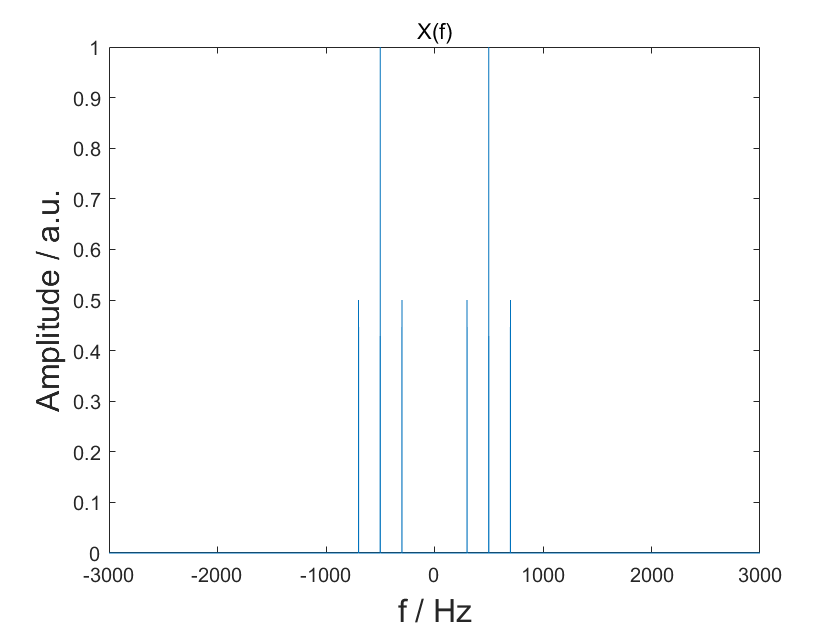
\includegraphics[width=0.45\textwidth]{Assignment-1-Problem-5-X(f).png}}
        \subfigure[Spectrum after the sampling: $X_{\delta}(f)$]{
        \label{5-Xdelta(f)}
        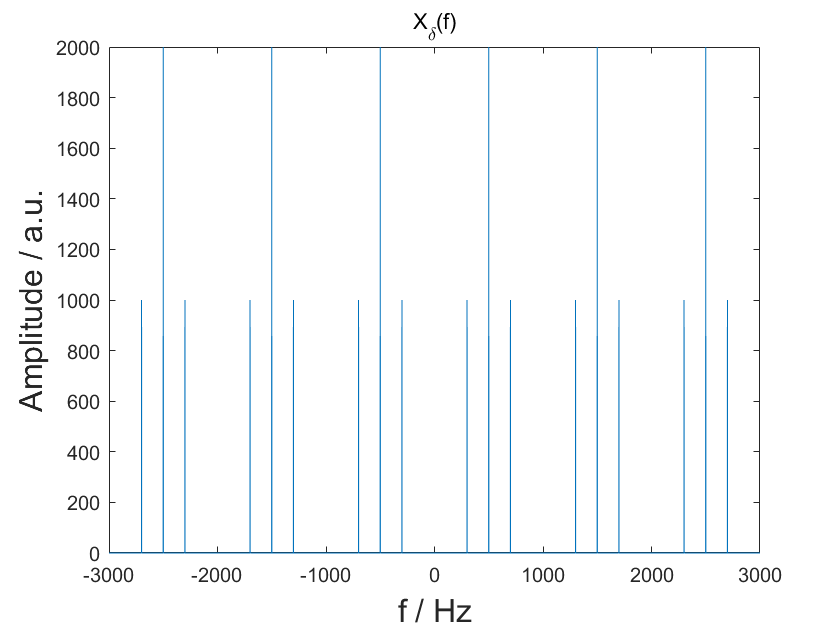
\includegraphics[width=0.45\textwidth]{Assignment-1-Problem-5-Xdelta(f).png}}
        \caption{}
        \label{5}
    \end{figure}
    According to the sampling theorem, the range of permissible cutoff frequencies for the ideal lowpass filter to reconstruct the signal is $700\text{Hz}<f_c<1300$Hz and the minimum allowable sampling frequency is $1400$Hz.
\end{sol}

\begin{prob}
    \begin{itemize}
        \item[1)] Express the spectrum $Y(f)$ of
        \[
            y(t)=x(t)\cos(400\pi t)+\hat{x}(t)\sin(400\pi t)
        \]
        using the spectrum $X(f)$ of $x(t)$, where $\hat{x}(t)$ is the Hilbert transform of $x(t)$. (5 pts)
        \item[2)] if $x(t)=\sinc(t)$, sketch $Y(f)$. (5 pts)
    \end{itemize}
\end{prob}
\begin{sol}
    \begin{itemize}
        \item[1)] The spectrum of $y(t)$ is
        \begin{align}
            \notag Y(f)=&\mathscr{F}[y(t)]=\mathscr{F}[x(t)\cos(400\pi t)+\hat{x}(t)\sin(400\pi t)]\\
            \notag=&\mathscr{F}\left[x(t)\frac{e^{j400\pi t}+e^{-j400\pi t}}{2}\right]+\mathscr{F}\left\{\mathscr{F}^{-1}[-j\sgn(f)X(f)]\frac{e^{j400\pi t}-e^{-j400\pi t}}{2j}\right\}\\
            =&\frac{1}{2}X(f-200)+\frac{1}{2}X(f+200)-\frac{1}{2}\sgn(f-200)X(f-200)+\frac{1}{2}\sgn(f+200)X(f+200)
        \end{align}
        \item[2)] If $x(t)=\sinc(t)$, then
        \begin{align}
            X(f)=\Pi(f)
        \end{align}
        and
        \begin{align}
            Y(f)=\frac{1}{2}\Pi(f-200)+\frac{1}{2}\Pi(f+200)-\frac{1}{2}\sgn(f-200)\Pi(f-200)+\frac{1}{2}\sgn(f+200)\Pi(f+200),
        \end{align}
        as shown in figure \ref{6}.
        \begin{figure}[h]
            \centering
            \subfigure[Overall view of $Y(f)$]{
            \label{6-Y(f)}
            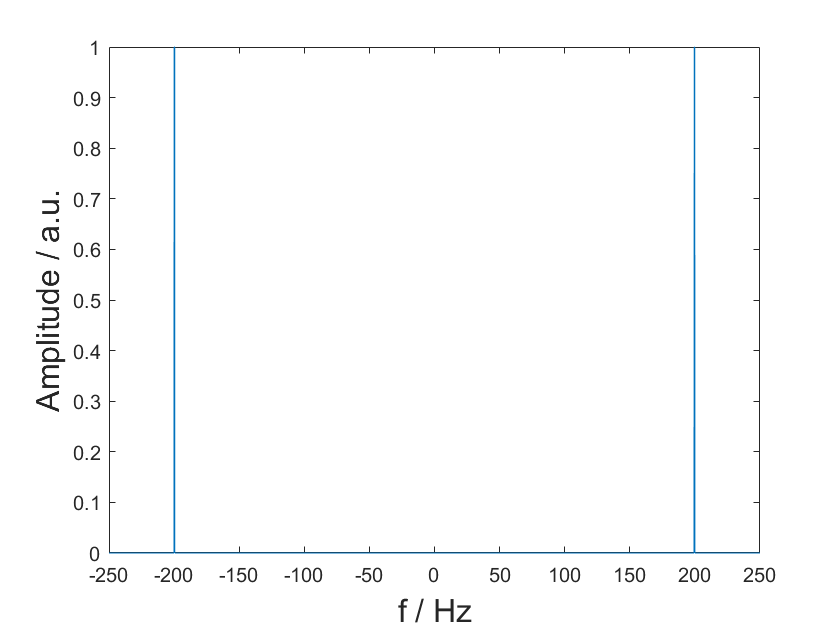
\includegraphics[width=0.6\textwidth]{Assignment-1-Problem-6-Y(f).png}}
            \subfigure[$Y(f)$ near $-200$]{
            \label{6-Y(f)near-200}
            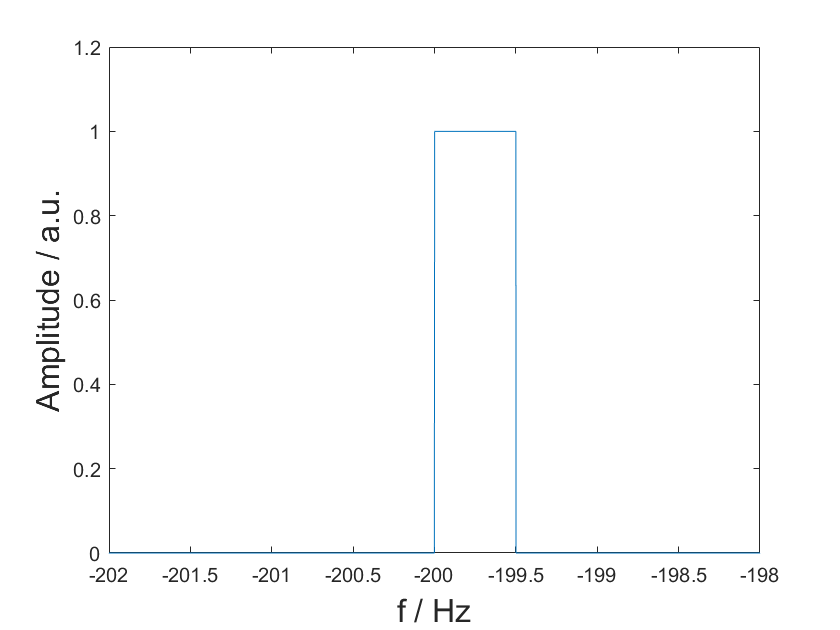
\includegraphics[width=0.4\textwidth]{Assignment-1-Problem-6-Y(f)near-200.png}}
            \subfigure[$Y(f)$ near $+200$]{
            \label{6-Y(f)near200}
            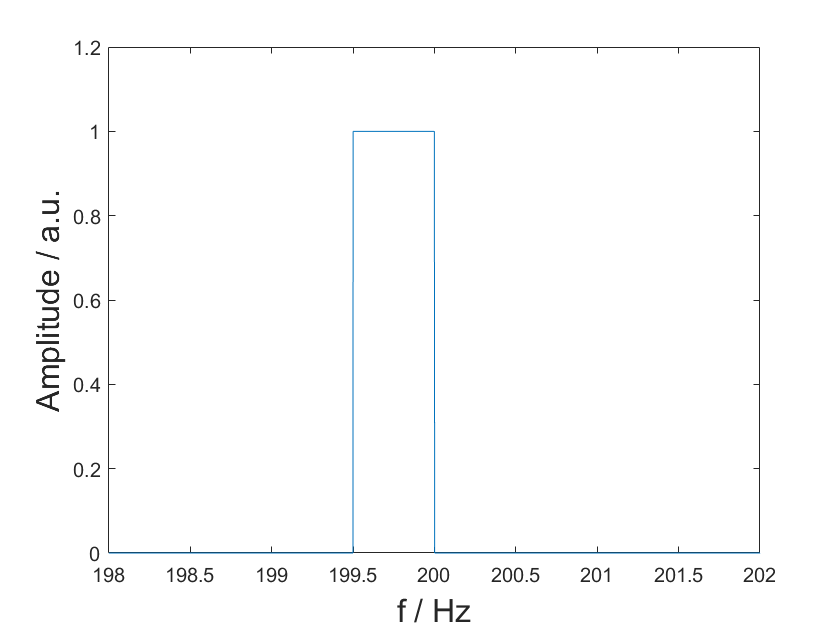
\includegraphics[width=0.4\textwidth]{Assignment-1-Problem-6-Y(f)near200.png}}
            \caption{Spectrum of $y(t)$: $Y(f)$}
            \label{6}
        \end{figure}
    \end{itemize}
\end{sol}

\begin{prob}
    Consider $x(t)=2\cos(60\pi t)$, the reference frequency $f_0=40$ Hz. Calculate the following signals.
    \begin{itemize}
        \item[a)] The Hilbert transform of $x(t)$, i.e., $\hat{x}(t)$.
        \item[b)] The analytic signal $x_p(t)$.
        \item[c)] The complex envelope of $x(t)$, i.e., $\tilde{x}(t)$.
        \item[d)] The inphase and quadrature component of $x(t)$, i.e., $x_R(t)$ and $x_I(t)$.\\
        (Please refer to Lecture 2, Slide 36 or Page 88 of reference textbook, we will learn this in the next class. I am sorry for the lagging.)
        \item[e)] Determine and plot the spectrum of the following signals:
        \begin{itemize}
            \item[i.] $x_1(t)=\frac{2}{3}x(t)+\frac{1}{3}j\hat{x}(t)$
            \item[ii.] $x_2(t)=\left[\frac{1}{5}x(t)+\frac{4}{5}j\hat{x}(t)\right]e^{j2\pi f_0t}$
        \end{itemize}
    \end{itemize}
\end{prob}
\begin{sol}
    \begin{itemize}
        \item[a)] The Fourier spectrum of $x(t)$ is
        \begin{align}
            \notag X(f)=\mathscr{F}[x(t)]=\delta(f-30)+\delta(f+30).
        \end{align}
        The spectrum of $x(t)$ after Hilbert transform is
        \begin{align}
            \hat{X}(f)=-j\sgn(f)X(f)=\delta(f-30)e^{-j\pi/2}+\delta(f+30)e^{j\pi/2}.
        \end{align}
        The Hilbert transform of $x(t)$ is
        \begin{align}
            \notag\hat{x}(t)=&\mathscr{F}^{-1}[\hat{X}(f)]=\mathscr{F}[\delta(f-30)e^{-j\pi/2}+\delta(f+30)e^{j\pi/2}]\\
            \notag=&e^{j60\pi t}e^{-j\pi/2}+e^{-j60\pi t}e^{j\pi/2}\\
            =&2\sin(60\pi t).
        \end{align}
        \item[b)] The analytic signal of $x(t)$ is
        \begin{align}
            x_p(t)=x(t)+j\hat{x}(t)=2\cos(60\pi t)+j2\sin(60\pi t)=2e^{j60\pi t}.
        \end{align}
        \item[c)] The complex envelope of $x(t)$ is
        \begin{align}
            \tilde{x}(t)=x_p(t)e^{-j2\pi 40t}=2e^{-j20\pi t}.
        \end{align}
        \item[d)] The inphase component of $x(t)$ is
        \begin{align}
            x_R(t)=\re[\tilde{x}(t)]=2\cos(20\pi t).
        \end{align}
        The quadrature component of $x(t)$ is
        \begin{align}
            x_I(t)=\im[\tilde{x}(t)]=2\sin(20\pi t).
        \end{align}
        \item[e)] 
        \begin{itemize}
            \item[i.] The spectrum of $x_1(t)$ is
            \begin{align}
                \notag X_1(f)=&\mathscr{F}[x_1(t)]=\mathscr{F}\left[\frac{2}{3}x(t)+\frac{1}{3}j\hat{x}(t)\right]\\
                \notag=&\frac{2}{3}X(f)+\frac{1}{3}j\hat{X}(f)\\
                \notag=&\frac{2}{3}[\delta(f-30)+\delta(f+30)]+\frac{1}{3}j\left[\delta(f-30)e^{-j\pi/2}+\delta(f+30)e^{j\pi/2}\right]\\
                =&\delta(f-30)+\frac{1}{3}\delta(f+30).
            \end{align}
            Its amplitude spectrum is
            \begin{align}
                \abs{X_1(f)}=\delta(f-30)+\frac{1}{3}\delta(f+30),
            \end{align}
            and angular spectrum is
            \begin{align}
                \theta_1(f)=0.
            \end{align}
            as shown in figure \ref{7-X1}.
            \begin{figure}[h]
                \centering
                \subfigure[$\abs{X_1(f)}$]{
                \label{7-X1(f)}
                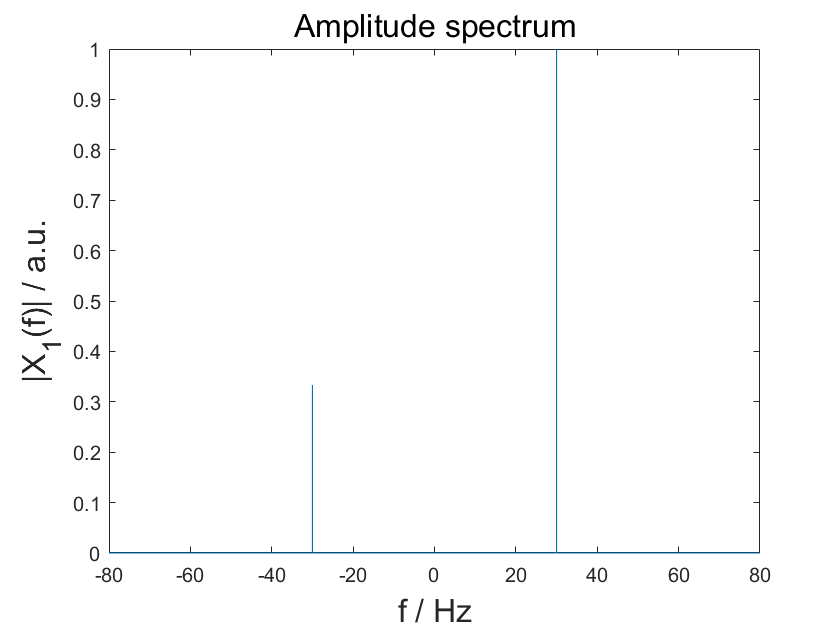
\includegraphics[width=0.45\textwidth]{Assignment-1-Problem-7-X1(f).png}}
                \subfigure[$\abs{\theta_1(f)}$]{
                \label{y-theta1(f)}
                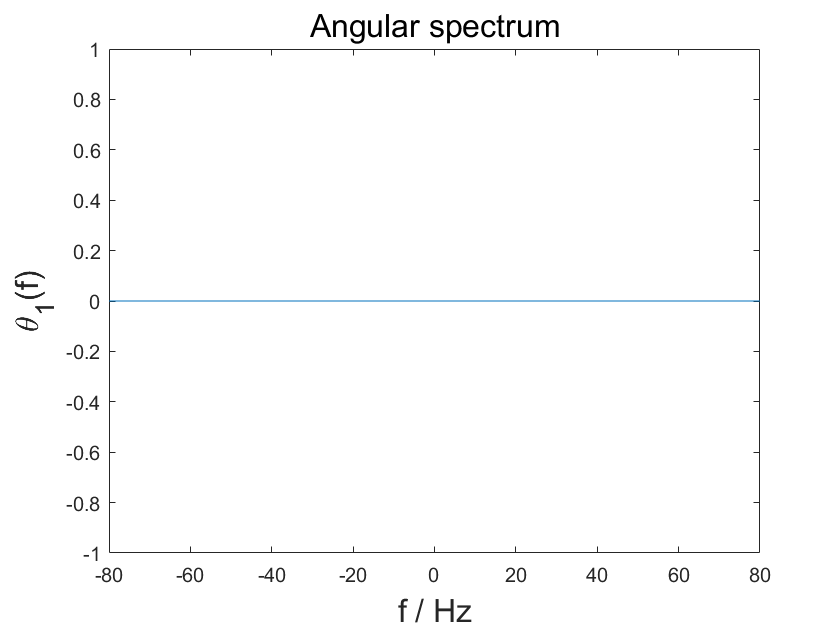
\includegraphics[width=0.45\textwidth]{Assignment-1-Problem-7-theta1(f).png}}
                \caption{Spectrum of $x_1(t)$}
                \label{7-X1}
            \end{figure}
            \item[ii.] The Fourier transform of $\left[\frac{1}{5}x(t)+\frac{4}{5}j\hat{x}(t)\right]$ is
            \begin{align}
                \notag\mathscr{F}\left[\frac{1}{5}x(t)+\frac{4}{5}j\hat{x}(t)\right]=&\frac{1}{5}X(f)+\frac{4}{5}j\hat{X}(f)\\
                \notag=&\frac{1}{5}[\delta(f-30)+\delta(f+30)]+\frac{4}{5}j\left[\delta(f-30)e^{-j\pi/2}+\delta(f+30)e^{j\pi/2}\right]\\
                =&\delta(f-30)-\frac{3}{5}\delta(f+30).
            \end{align}
            Using the frequency shifting property, we get the spectrum of $x_2(t)$:
            \begin{align}
                X_1(f)=\mathscr{F}[x_2(t)]=\mathscr{F}\left\{\left[\frac{1}{5}x(t)+\frac{4}{5}j\hat{x}(t)\right]e^{j2\pi f_0t}\right\}=\delta(f-f_0-30)-\frac{3}{5}\delta(f-f_0+30).
            \end{align}
            Its amplitude spectrum is
            \begin{align}
                \abs{X_1(f)}=\delta(f-f_0-30)-\frac{3}{5}\delta(f-f_0+30)=\delta(f-70)-\frac{3}{5}\delta(f-10),
            \end{align}
            and angular spectrum is
            \begin{align}
                \theta_2(f)=0,
            \end{align}
            as shown in figure \ref{7-X2}.
			\begin{figure}[h]
                \centering
                \subfigure[$\abs{X_2(f)}$]{
                \label{7-X2(f)}
                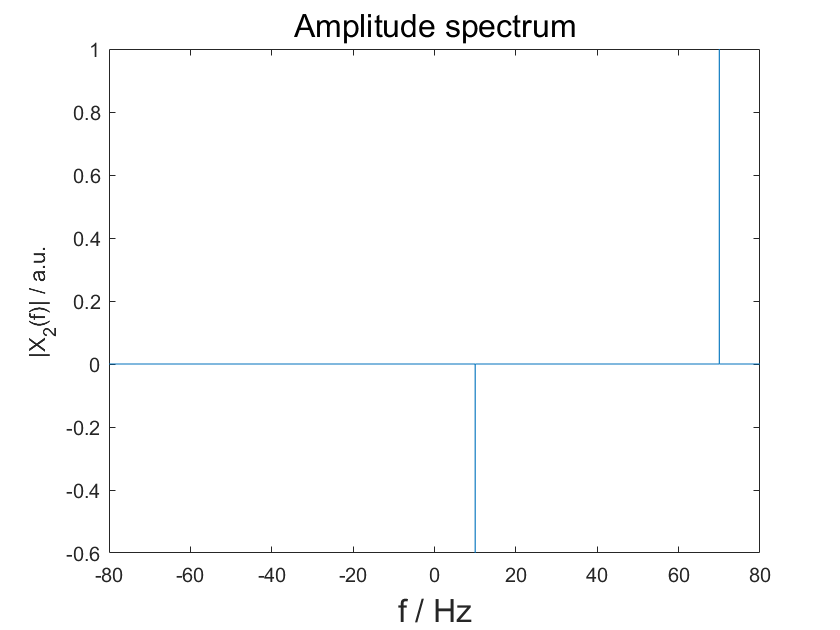
\includegraphics[width=0.45\textwidth]{Assignment-1-Problem-7-X2(f).png}}
                \subfigure[$\abs{\theta_2(f)}$]{
                \label{7-theta2(f)}
                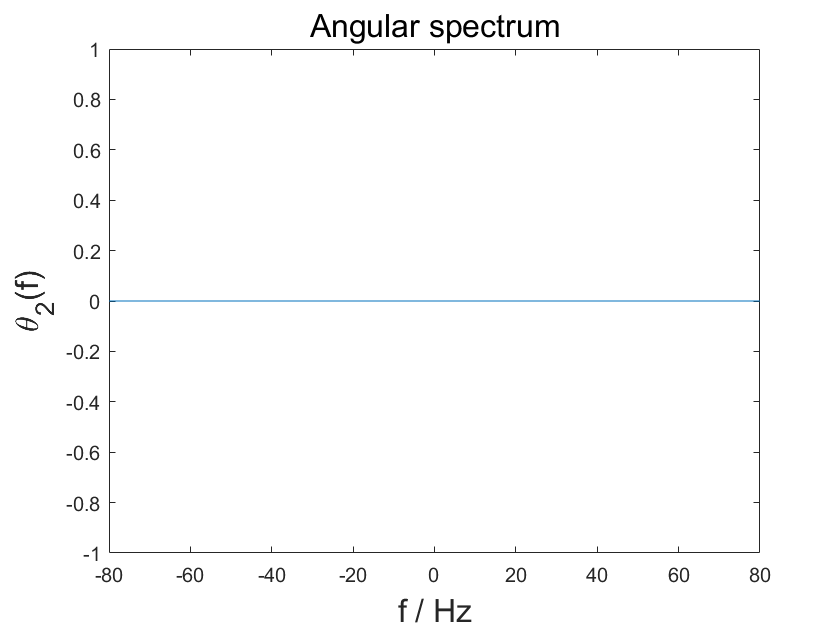
\includegraphics[width=0.45\textwidth]{Assignment-1-Problem-7-theta2(f).png}}
                \caption{Spectrum of $x_2(t)$}
                \label{7-X2}
            \end{figure}
        \end{itemize}
    \end{itemize}
\end{sol}
\end{document}